\documentclass{article}
\usepackage[utf8]{inputenc}
	\addtolength{\oddsidemargin}{-.875in}
		\addtolength{\textheight}{0.5in}
\usepackage{graphicx}
\usepackage[table,xcdraw]{xcolor}
\usepackage{amsmath}
\title{CON101: Digital Divide and Net Neutrality}
\author{ANIRUDHA KULKARNI \\ 2019CS50421}
\date{October 2020}
\usepackage{graphics}
\usepackage{hyperref}
\usepackage[export]{adjustbox}
\usepackage[table,xcdraw]{xcolor}
\usepackage[a4paper, total={6in, 8in}]{geometry}
\begin{document}

\maketitle

\section{Introduction}
To understand differences in network speed with change in location, Time of day, Network provider and Mobile data vs Broadband different measurement data was collected from 5th October 2020 to 11th October 2020 on group basis involving students:\\
% \usepackage{colortbl}


\begin{table}[hbt!]
\centering
\arrayrulecolor{black}
\begin{tabular}{!{\color{black}\vrule}l!{\color{black}\vrule}l!{\color{black}\vrule}l!{\color{black}\vrule}l!{\color{black}\vrule}l!{\color{black}\vrule}} 
\hline
Sr. & Name                    & Entry Number & Network             & Location                                  \\ 
\hline
1       & Anirudha
  Kulkarni     & 2019CS50421  & Airtel , Jio        & Maharashtra 18.4088°
  N, 76.5604° E      \\ 
\hline
2       & Prakhar
  Aggarwal~~~~~ & 2019CS50441  & Broadband,
  Airtel & Panjab 30°20'50.0"N
  76°21'35.9"E        \\ 
\hline
3       & Pratyush Saini          & 2019CS10444  & Jio                 & Uttarakhand 30.387679°
  N, 78.091759° E  \\
\hline
\end{tabular}
\arrayrulecolor{black}
\end{table}\\
Measurement provider: Speed test by Ookla: \url{https://www.speedtest.net/}  \\
Data sheet: \url{https://docs.google.com/spreadsheets/d/17NJ1JOZWhGQVvP1dccnpMJymj5wIGmCacr_hu0QVOP8/edit?usp=sharing}\\
Window of measurement:
\begin{itemize}
  \item  Morning: 8-9 AM
  \item  Evening: 10-11.59 PM
\end{itemize}
\pagebreak
\section{Upload and Download}
\subsection{Network1}



\begin{table}[hbt!]
\centering
\arrayrulecolor{black}
\begin{tabular}{!{\color[rgb]{0.8,0.8,0.8}\vrule}l!{\color{black}\vrule}l!{\color[rgb]{0.8,0.8,0.8}\vrule}l!{\color[rgb]{0.8,0.8,0.8}\vrule}l!{\color[rgb]{0.8,0.8,0.8}\vrule}l!{\color[rgb]{0.8,0.8,0.8}\vrule}} 
\hline
     &         & \multicolumn{3}{l!{\color[rgb]{0.8,0.8,0.8}\vrule}}{Anirudha Airtel}  \\ 
\hline
Date & Slot    & ping (ms) & Download (Mbps) & Upload (Mbps)                           \\ 
\hline
5    & Morning & 39        & 20              & 2.01                                    \\ 
\hline
5    & Evening & 34        & 14.84           & 1.86                                    \\ 
\hline
6    & Morning & 59        & 35.89           & 2.53                                    \\ 
\hline
6    & Evening & 37        & 29.46           & 1.18                                    \\ 
\hline
7    & Morning & 60        & 30.52           & 1.79                                    \\ 
\hline
7    & Evening & 35        & 24.21           & 1.42                                    \\ 
\hline
8    & Morning & 42        & 20.24           & 1.89                                    \\ 
\hline
8    & Evening & 30        & 10.69           & 2.12                                    \\ 
\hline
9    & Morning & 31        & 16.85           & 1.23                                    \\ 
\hline
9    & Evening & 34        & 20.56           & 2.16                                    \\ 
\hline
10   & Morning & 36        & 12.89           & 1.64                                    \\ 
\hline
10   & Evening & 37        & 12.53           & 2.78                                    \\ 
\hline
11   & Morning & 57        & 34.26           & 1.49                                    \\ 
\hline
11   & Evening & 37        & 13.45           & 2.43                                    \\
\hline
\end{tabular}
\arrayrulecolor{black}
\end{table}
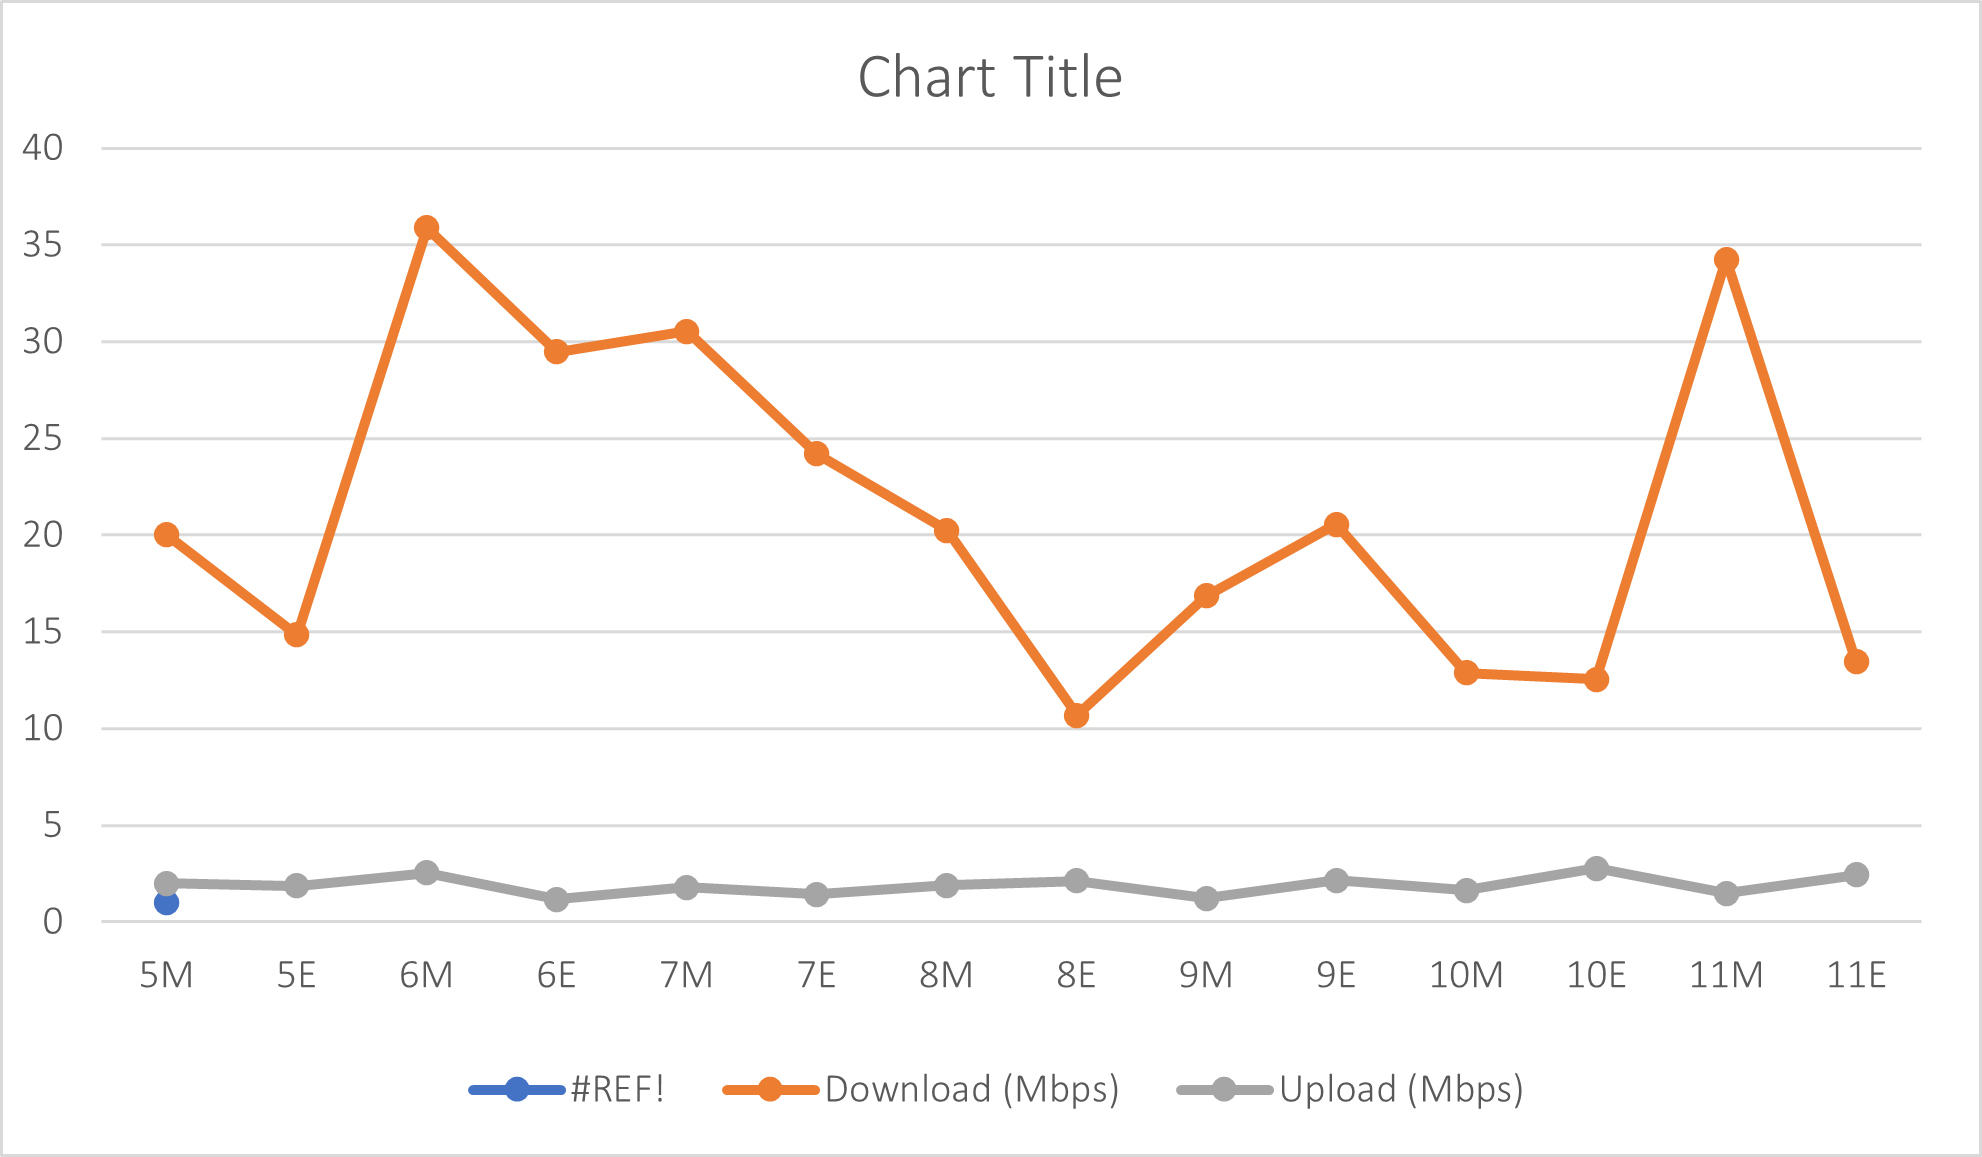
\includegraphics{aniairtel.png}
%end part 1
\pagebreak
\subsection{Network 2}
% \usepackage{colortbl}
\begin{table}[hbt!]
\centering
\arrayrulecolor{black}
\begin{tabular}{!{\color[rgb]{0.8,0.8,0.8}\vrule}l!{\color{black}\vrule}l!{\color[rgb]{0.8,0.8,0.8}\vrule}l!{\color[rgb]{0.8,0.8,0.8}\vrule}l!{\color[rgb]{0.8,0.8,0.8}\vrule}l!{\color[rgb]{0.8,0.8,0.8}\vrule}} 
\hline
     &         & \multicolumn{3}{l!{\color[rgb]{0.8,0.8,0.8}\vrule}}{Anirudha Jio}  \\ 
\hline
Date & Slot    & ping (ms) & Download (Mbps) & Upload (Mbps)                        \\ 
\hline
5    & Morning & 80        & 10.45           & 1.45                                 \\ 
\hline
5    & Evening & 82        & 16.5            & 2.1                                  \\ 
\hline
6    & Morning & 85        & 3.48            & 2.91                                 \\ 
\hline
6    & Evening & 81        & 5.7             & 4.33                                 \\ 
\hline
7    & Morning & 70        & 1.57            & 0.63                                 \\ 
\hline
7    & Evening & 55        & 5.48            & 1.12                                 \\ 
\hline
8    & Morning & 82        & 4.59            & 0.76                                 \\ 
\hline
8    & Evening & 77        & 3.5             & 0.65                                 \\ 
\hline
9    & Morning & 88        & 4.16            & 1.84                                 \\ 
\hline
9    & Evening & 65        & 8.46            & 4.56                                 \\ 
\hline
10   & Morning & 84        & 3.15            & 1.36                                 \\ 
\hline
10   & Evening & 70        & 6.45            & 3.78                                 \\ 
\hline
11   & Morning & 76        & 2.46            & 0.98                                 \\ 
\hline
11   & Evening & 79        & 7.26            & 1.79                                 \\
\hline
\end{tabular}
\arrayrulecolor{black}
\end{table}
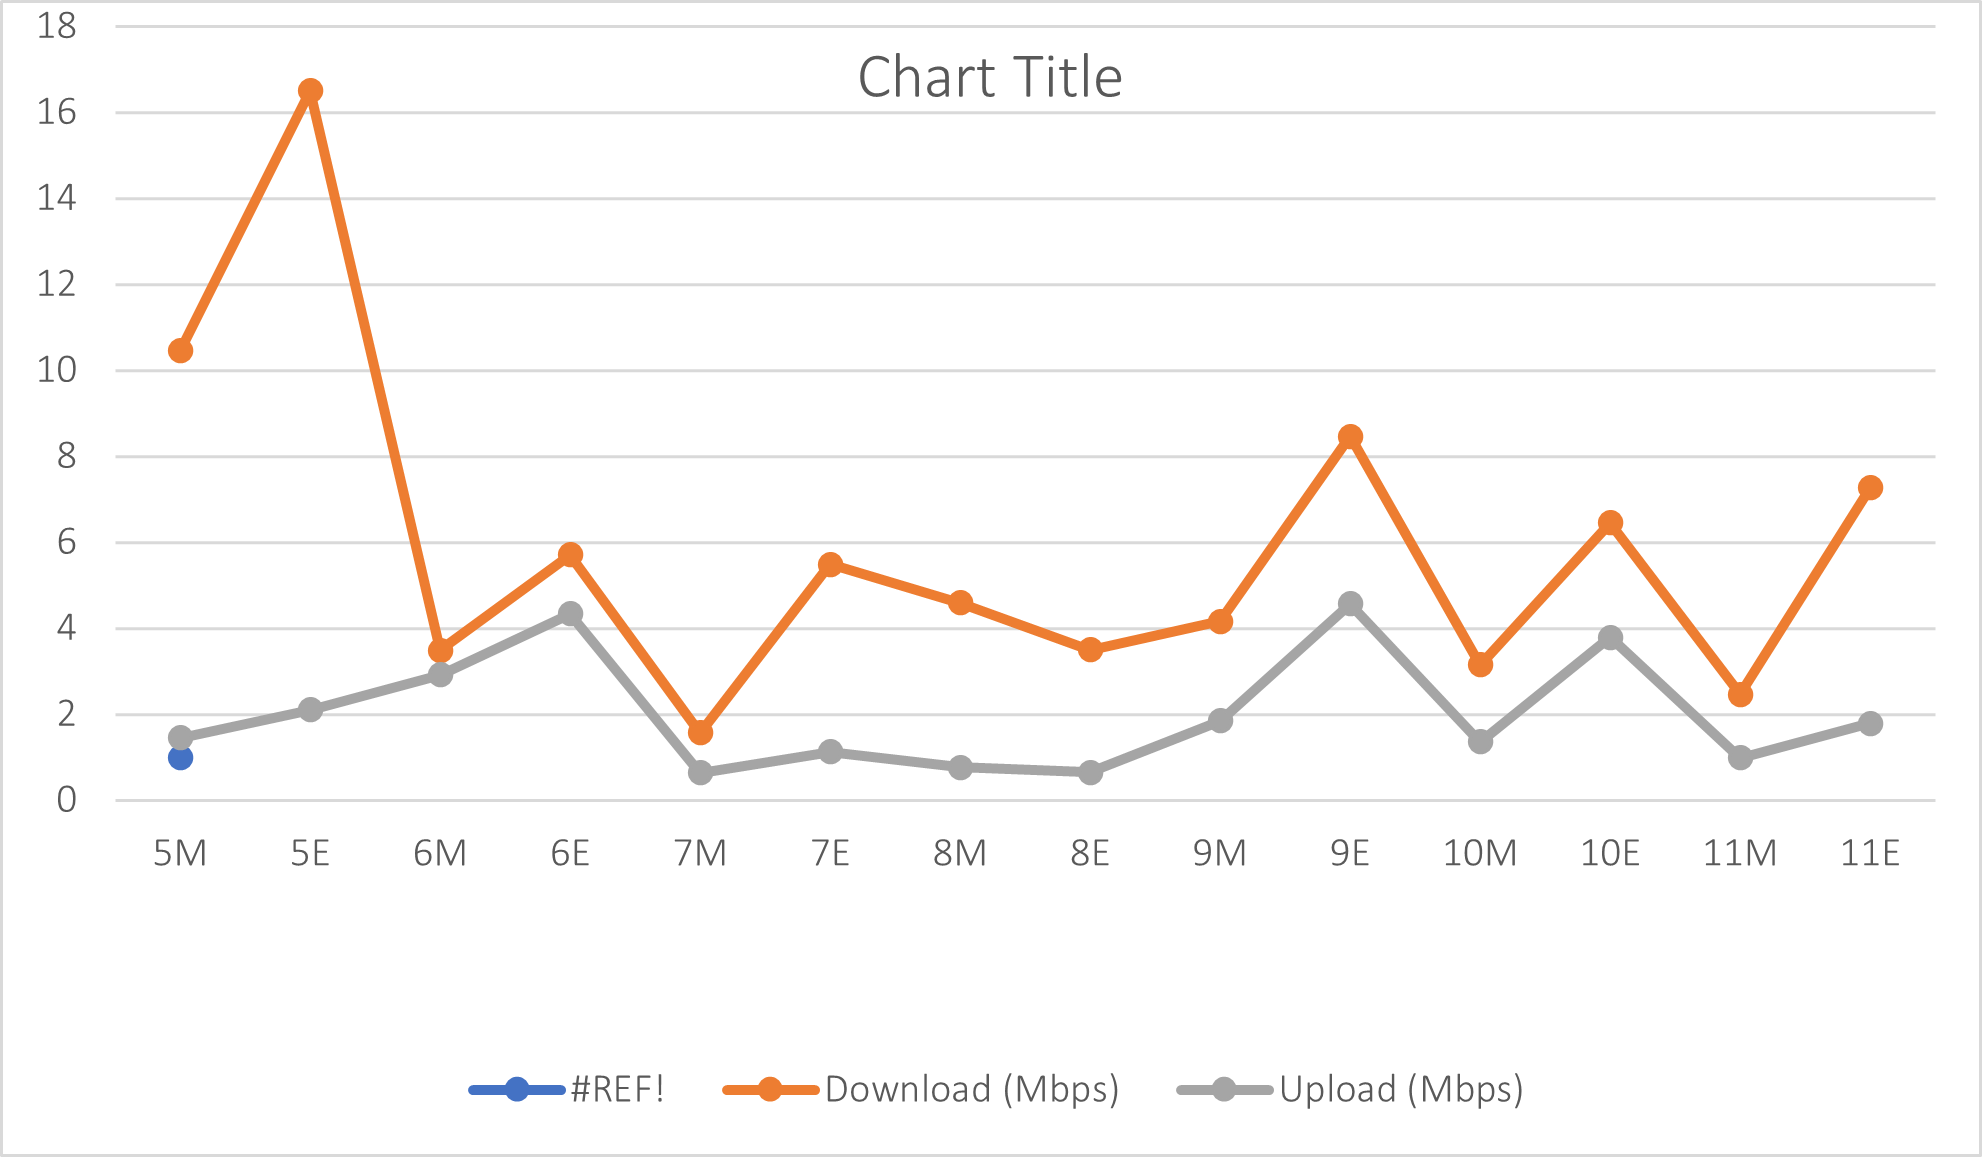
\includegraphics{anijio.png}
\pagebreak
\subsection{Network 3}
%%%%%%%%%%%%%%%%%%%
% \usepackage{colortbl}


\begin{table}[hbt!]
\centering
\arrayrulecolor{black}
\begin{tabular}{!{\color[rgb]{0.8,0.8,0.8}\vrule}l!{\color{black}\vrule}l!{\color[rgb]{0.8,0.8,0.8}\vrule}l!{\color[rgb]{0.8,0.8,0.8}\vrule}l!{\color[rgb]{0.8,0.8,0.8}\vrule}l!{\color[rgb]{0.8,0.8,0.8}\vrule}} 
\hline
     &         & \multicolumn{3}{l!{\color[rgb]{0.8,0.8,0.8}\vrule}}{Prakhar Broadband}  \\ 
\hline
Date & Slot    & ping (ms) & Download (Mbps) & Upload (Mbps)                             \\ 
\hline
5    & Morning & 7         & 22.9            & 23.7                                      \\ 
\hline
5    & Evening & 8         & 27.2            & 16.7                                      \\ 
\hline
6    & Morning & 8         & 36.5            & 25.4                                      \\ 
\hline
6    & Evening & 7         & 34.3            & 19.9                                      \\ 
\hline
7    & Morning & 7         & 43.2            & 15.7                                      \\ 
\hline
7    & Evening & 7         & 45.1            & 34.7                                      \\ 
\hline
8    & Morning & 7         & 32.5            & 10.1                                      \\ 
\hline
8    & Evening & 7         & 37.7            & 19.4                                      \\ 
\hline
9    & Morning & 7         & 33.4            & 13.5                                      \\ 
\hline
9    & Evening & 8         & 35.4            & 21.3                                      \\ 
\hline
10   & Morning & 7         & 30.2            & 12.3                                      \\ 
\hline
10   & Evening & 7         & 39.8            & 17.4                                      \\ 
\hline
11   & Morning & 7         & 26.7            & 15.2                                      \\ 
\hline
11   & Evening & 8         & 36.9            & 19.8                                      \\
\hline
\end{tabular}
\arrayrulecolor{black}
\end{table}
%%%%%%%%%%%%%%%%%%%%%%%%%%%
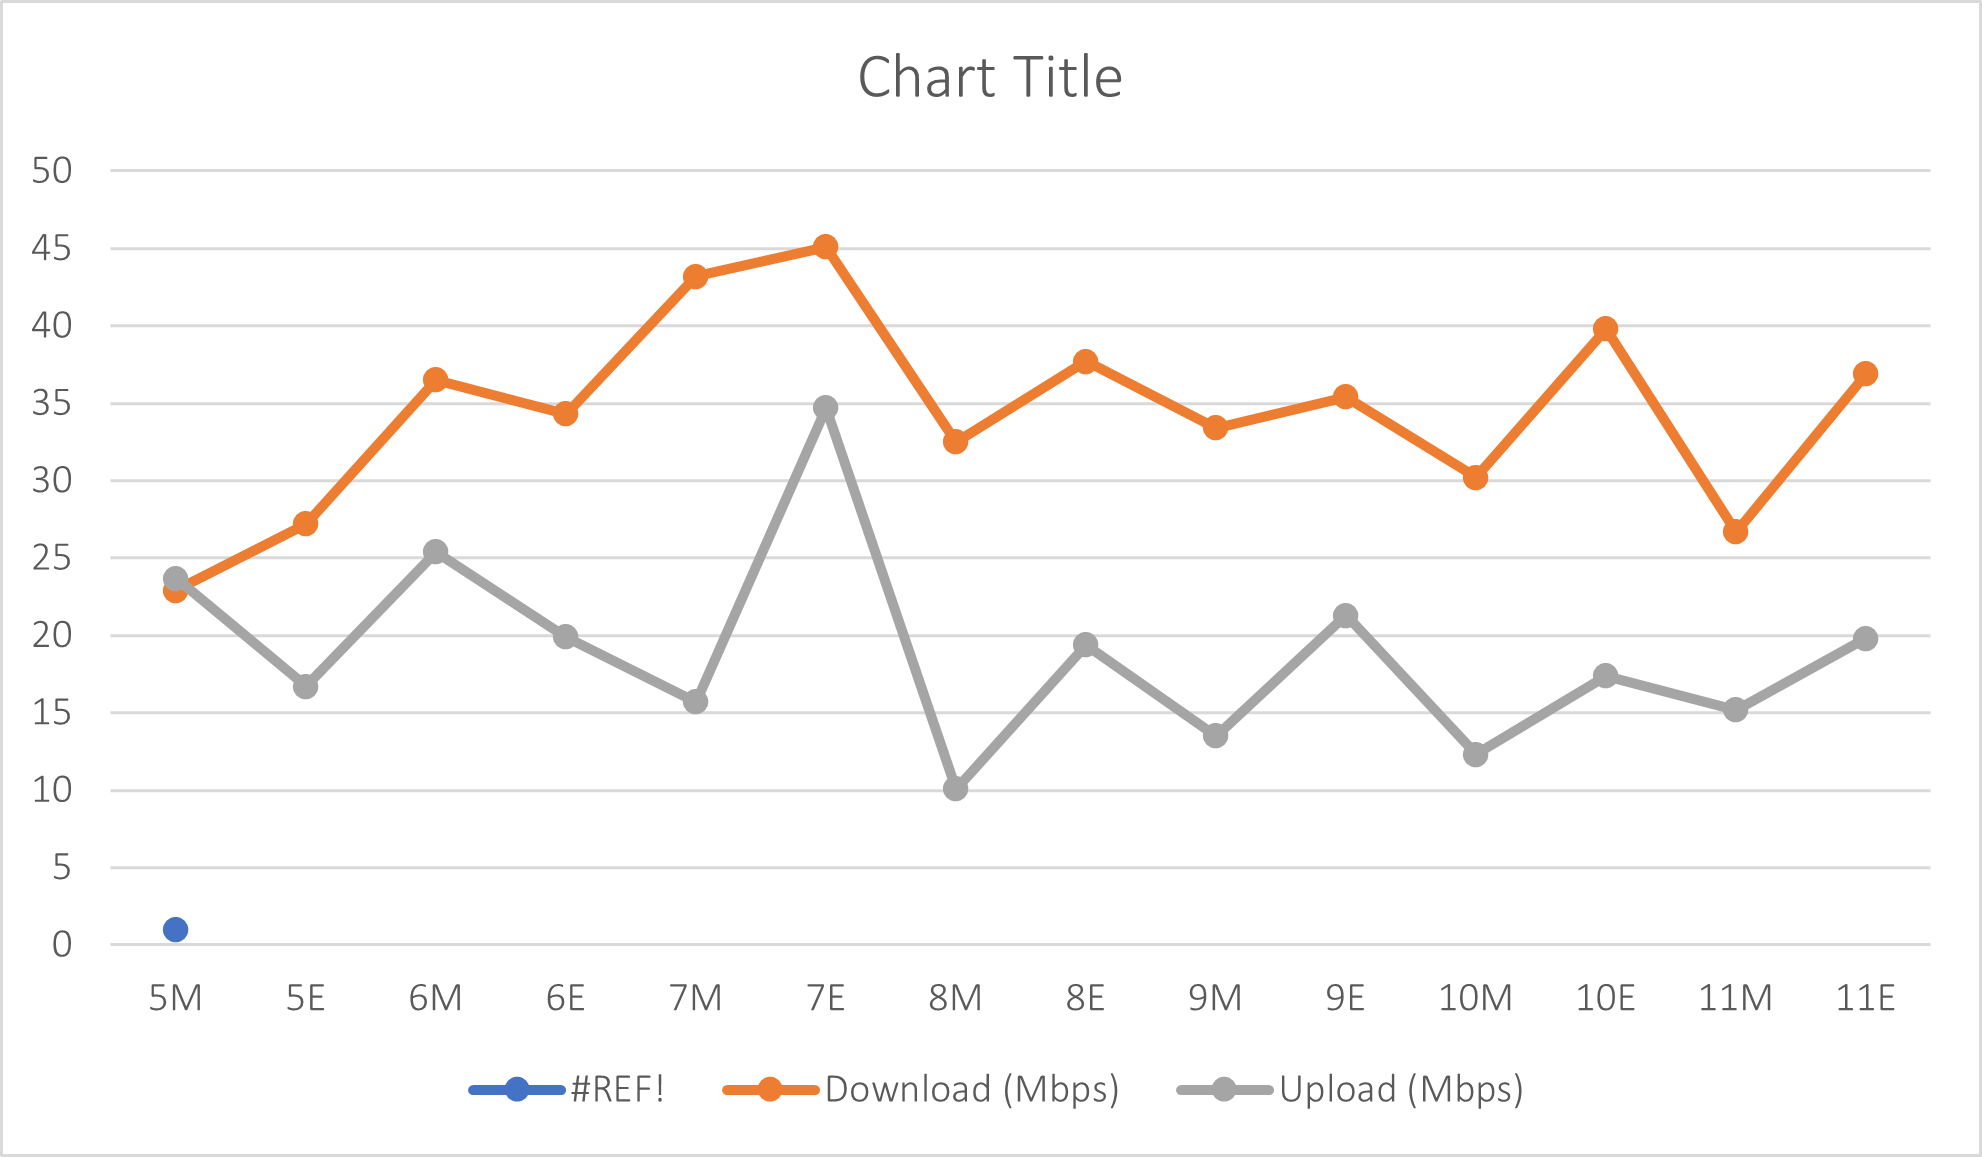
\includegraphics[]{prakharbroad.png}
\pagebreak
%%%%%%%%%%%%%%%
\subsection{Network 4}

% \usepackage{colortbl}


\begin{table}[hbt!]
\centering
\arrayrulecolor{black}
\begin{tabular}{!{\color[rgb]{0.8,0.8,0.8}\vrule}l!{\color{black}\vrule}l!{\color[rgb]{0.8,0.8,0.8}\vrule}l!{\color[rgb]{0.8,0.8,0.8}\vrule}l!{\color[rgb]{0.8,0.8,0.8}\vrule}l!{\color[rgb]{0.8,0.8,0.8}\vrule}} 
\hline
     &         & \multicolumn{3}{l!{\color[rgb]{0.8,0.8,0.8}\vrule}}{Prakhar Airtel}  \\ 
\hline
Date & Slot    & ping (ms) & Download (Mbps) & Upload (Mbps)                          \\ 
\hline
5    & Morning & 24        & 10.2            & 1.55                                   \\ 
\hline
5    & Evening & 37        & 22.9            & 5.48                                   \\ 
\hline
6    & Morning & 32        & 1.39            & 2.8                                    \\ 
\hline
6    & Evening & 20        & 7.5             & 2.58                                   \\ 
\hline
7    & Morning & 19        & 11.3            & 1.12                                   \\ 
\hline
7    & Evening & 20        & 23              & 5.77                                   \\ 
\hline
8    & Morning & 35        & 6.64            & 3.48                                   \\ 
\hline
8    & Evening & 23        & 16.4            & 5.15                                   \\ 
\hline
9    & Morning & 28        & 1.23            & 2.2                                    \\ 
\hline
9    & Evening & 26        & 17.5            & 5.11                                   \\ 
\hline
10   & Morning & 27        & 3.4             & 3.11                                   \\ 
\hline
10   & Evening & 24        & 20.2            & 4.8                                    \\ 
\hline
11   & Morning & 30        & 6.1             & 1.84                                   \\ 
\hline
11   & Evening & 29        & 18.4            & 6.12                                   \\ 
\hline
\end{tabular}
\arrayrulecolor{black}
\end{table}
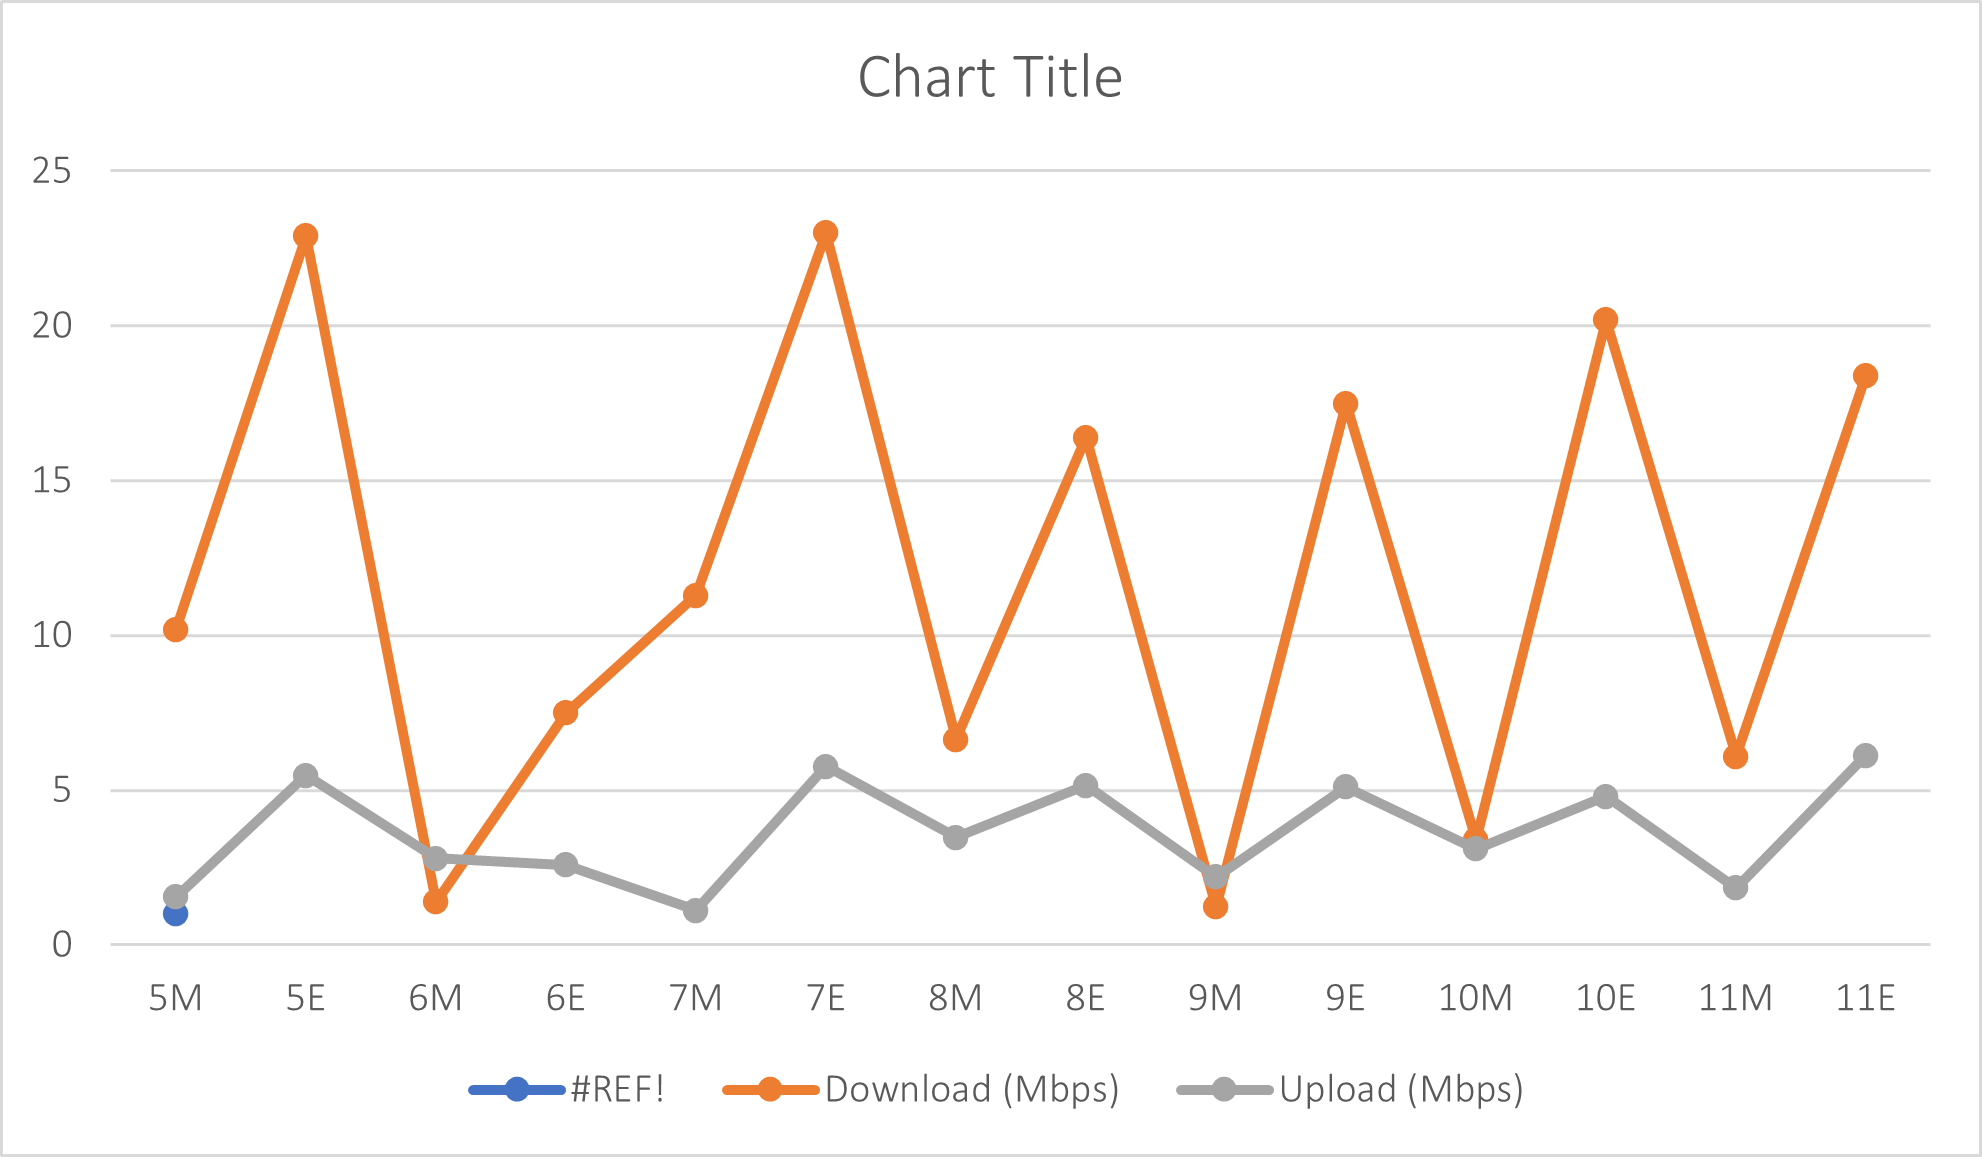
\includegraphics[]{prakharair.png}
\pagebreak
%%%%%%%%%%%%%%%%%%%%%
\subsection{Network 5}
% \usepackage{colortbl}


\begin{table}[hbt!]
\centering
\arrayrulecolor{black}
\begin{tabular}{!{\color[rgb]{0.8,0.8,0.8}\vrule}l!{\color{black}\vrule}l!{\color[rgb]{0.8,0.8,0.8}\vrule}l!{\color[rgb]{0.8,0.8,0.8}\vrule}l!{\color[rgb]{0.8,0.8,0.8}\vrule}l!{\color[rgb]{0.8,0.8,0.8}\vrule}} 
\hline
     &         & \multicolumn{3}{l!{\color[rgb]{0.8,0.8,0.8}\vrule}}{Pratyush JIO}  \\ 
\hline
Date & Slot    & ping (ms) & Download (Mbps) & Upload (Mbps)                        \\ 
\hline
5    & Morning & 53        & 8.8             & 3.71                                 \\ 
\hline
5    & Evening & 58        & 39.4            & 9.14                                 \\ 
\hline
6    & Morning & 41        & 32.7            & 9.73                                 \\ 
\hline
6    & Evening & 48        & 14.6            & 6.39                                 \\ 
\hline
7    & Morning & 30        & 33.4            & 8.21                                 \\ 
\hline
7    & Evening & 54        & 22              & 8.4                                  \\ 
\hline
8    & Morning & 30        & 23.4            & 8.6                                  \\ 
\hline
8    & Evening & 52        & 18.2            & 8.7                                  \\ 
\hline
9    & Morning & 29        & 18.5            & 8.9                                  \\ 
\hline
9    & Evening & 48        & 20.6            & 6.04                                 \\ 
\hline
10   & Morning & 36        & 19              & 7.43                                 \\ 
\hline
10   & Evening & 38        & 25.5            & 7.8                                  \\ 
\hline
11   & Morning & 38        & 23.6            & 7.86                                 \\ 
\hline
11   & Evening & 44        & 24              & 7.9                                  \\
\hline
\end{tabular}
\arrayrulecolor{black}
\end{table}
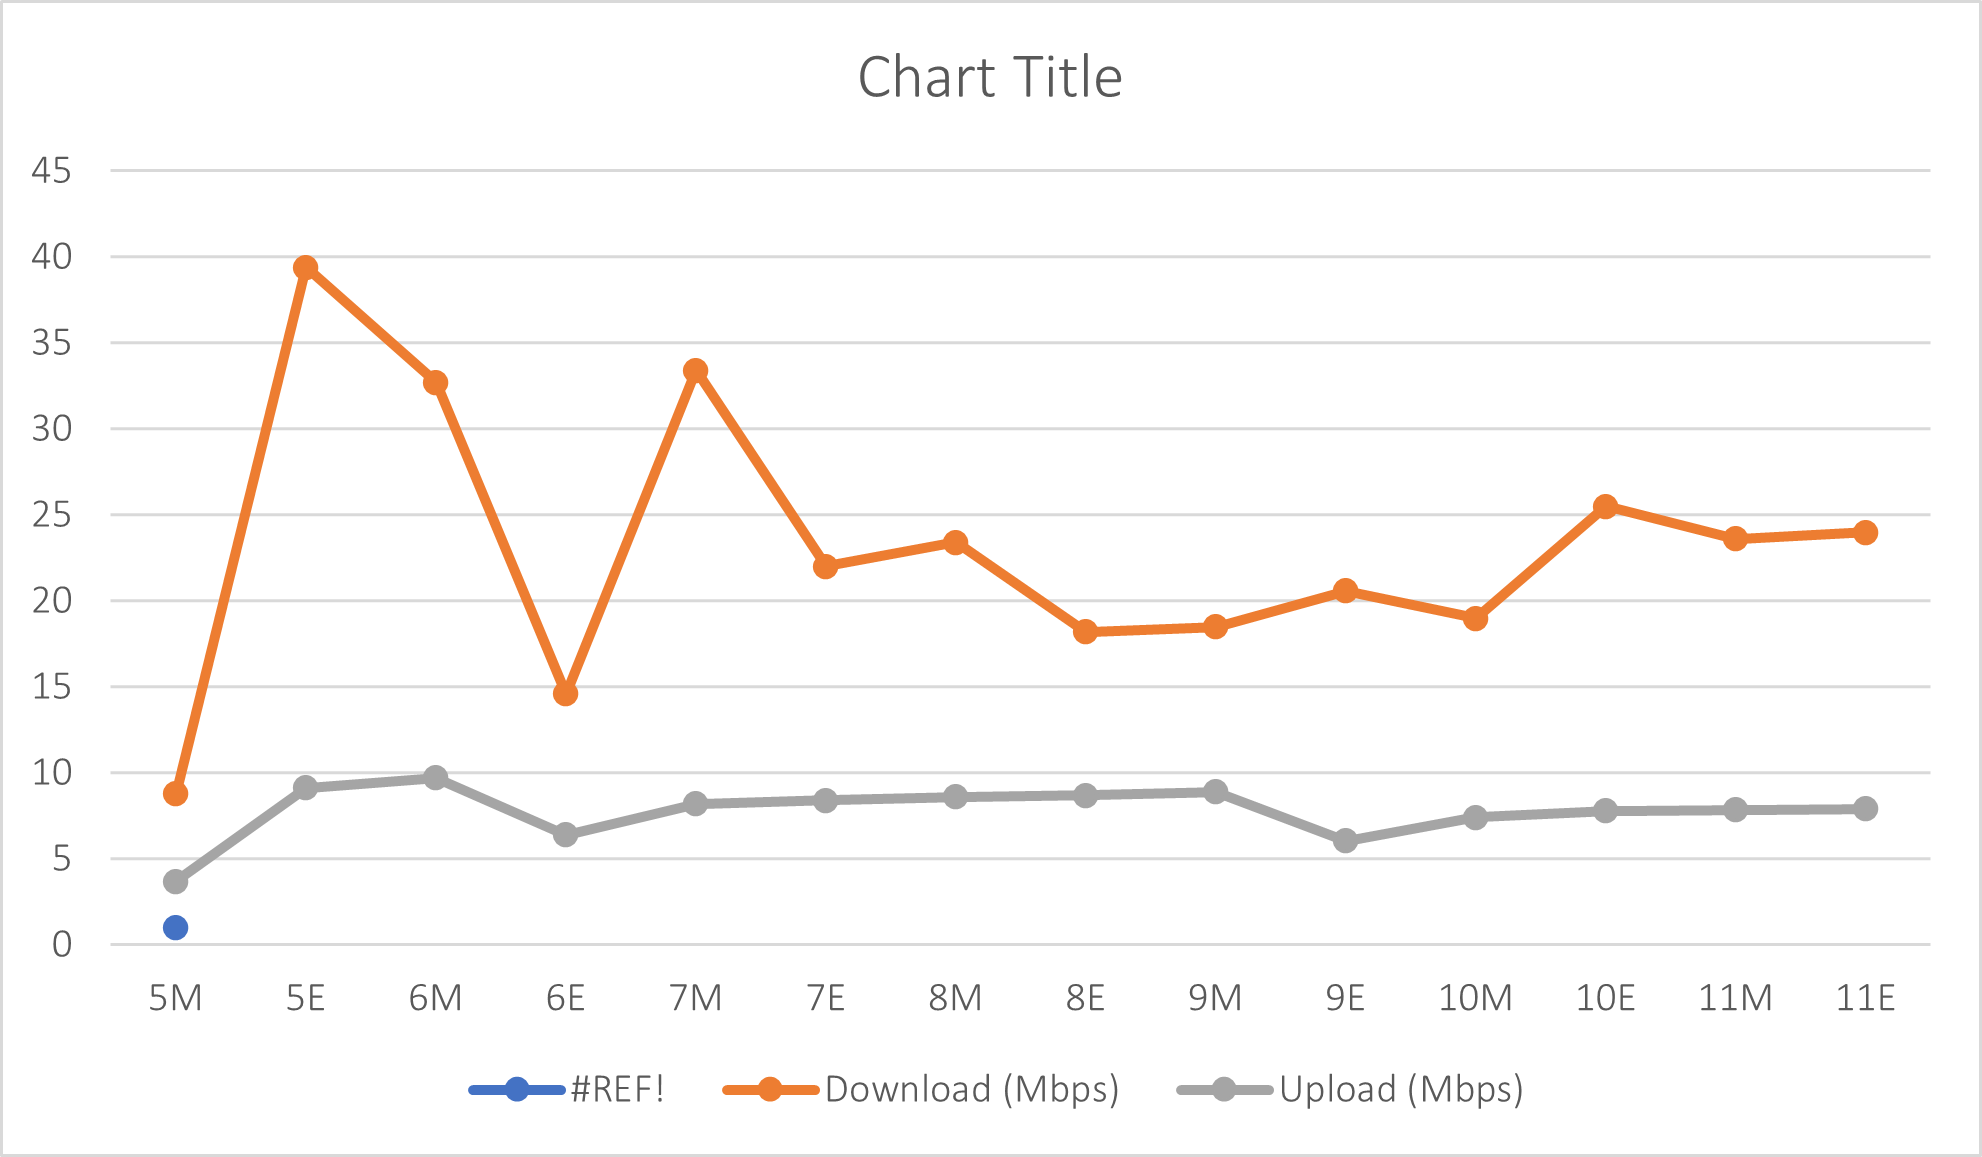
\includegraphics[]{prat.png}
\pagebreak
%%%%%%%%%%%%%%%%%%%%%%%
\section{Latency Comparison}
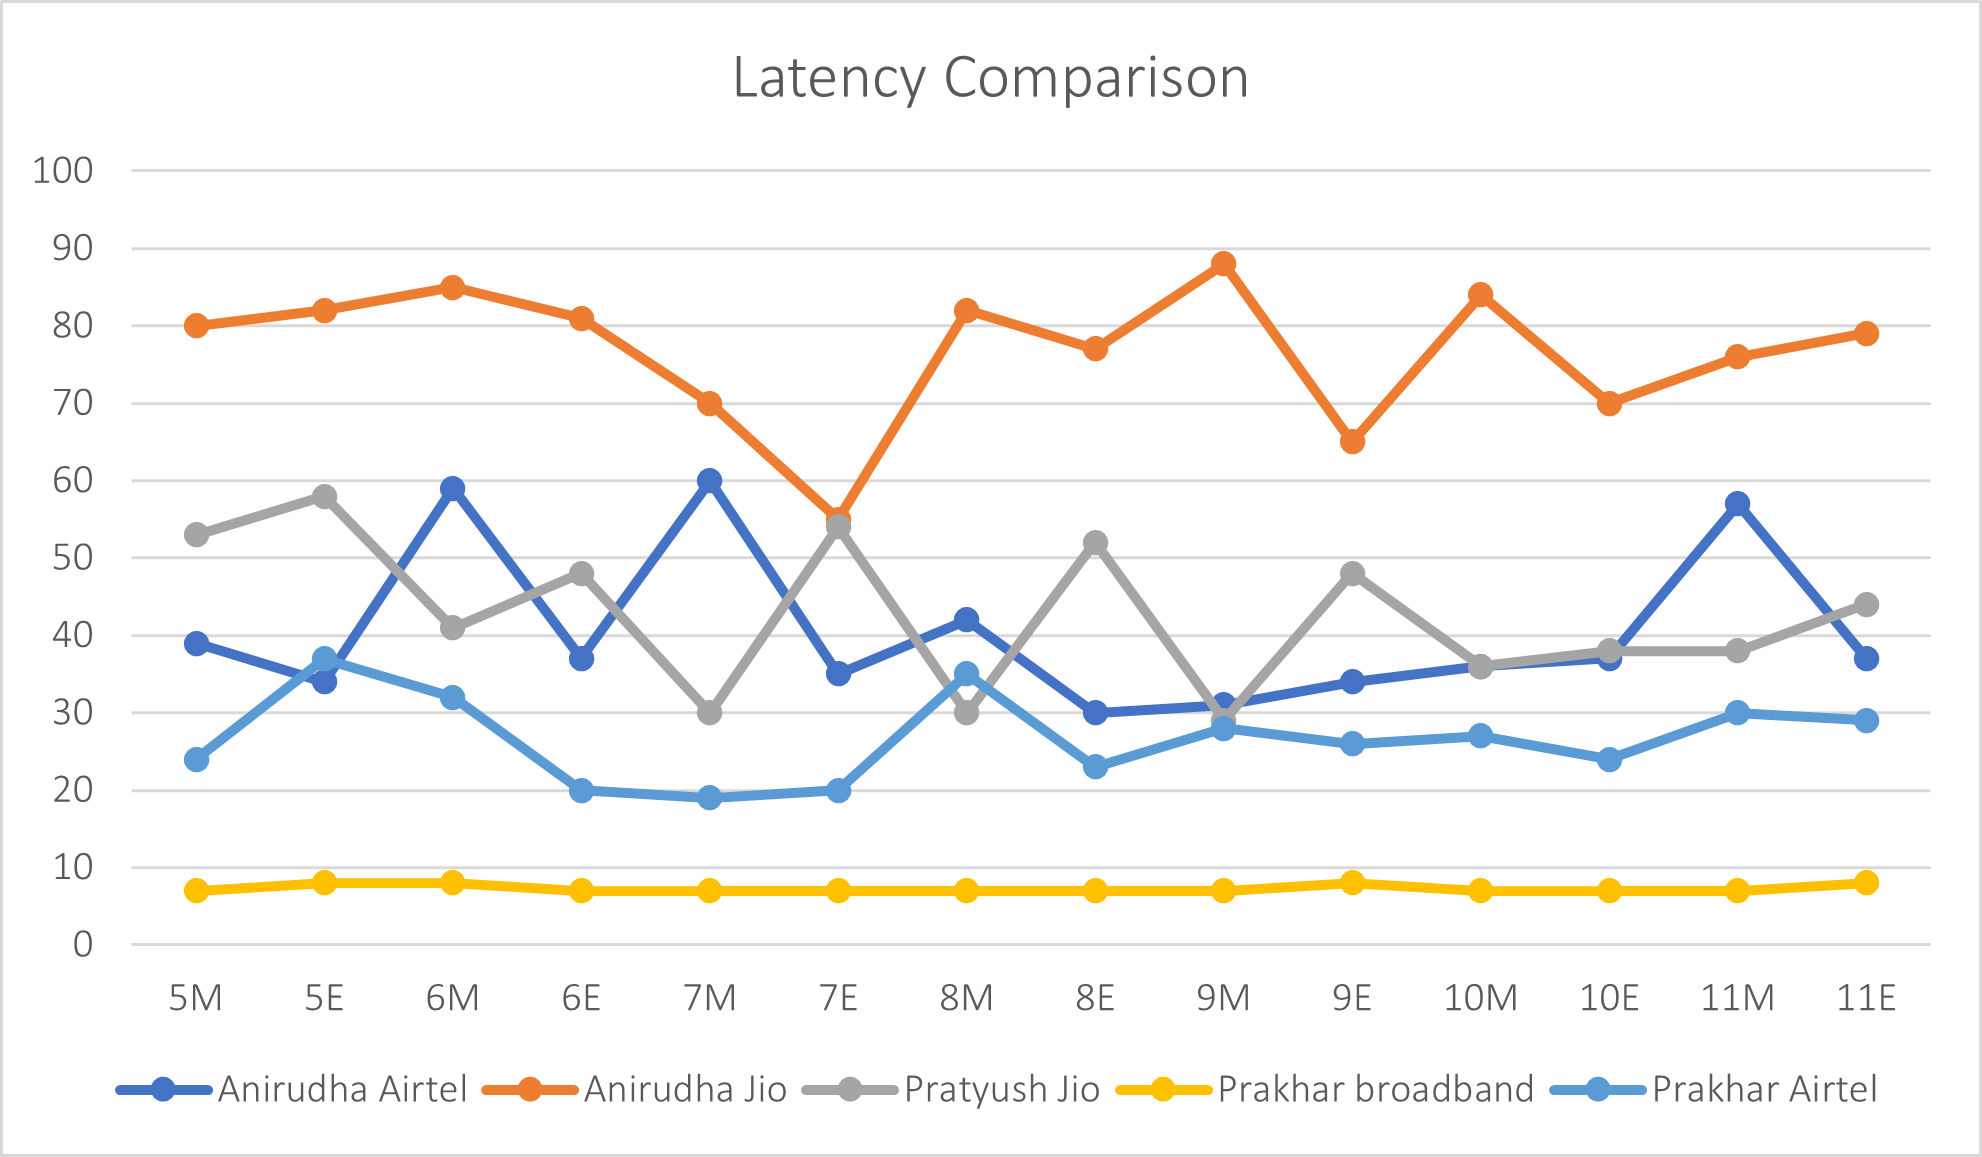
\includegraphics{latency.png}
\pagebreak
\section{Data Analysis}
As seen from data Broadband clearly performs much better than mobile networks in all of 3 aspects. Also network performance is much better in early morning than night. The sharp ups and downs in the graph indicates this fact. It can be attributed to lower traffic in morning compared to night. Also Airtel seems to perform slightly better than Jio in this measurements. Latency is much better in broadband than mobile networks which can be attributed to mobile nature of mobile networks. metropolitan cities compared small towns. It can be seen from network3/4 data (patiala) vs network 1 data (Latur).\\ But all the performances are much below the promised/ advertised performance. It might be due to high traffic than expected and/ or different measurement methodology.
\pagebreak
\section{Measurement Methodology used by Apps}
Internet speed is mainly determined by  3 aspects:
\begin{itemize}
    \item 1. Upload speed 
\item 2. Download speed
\item 3. Latency or ping.
\end{itemize}


A balance of all 3 determines overall experience.
\subsection{Upload speed}
Its measured by sending a small amount of data from user machine to remote server. The time taken is also measured and speed is calculated by amount of data transferred per unit secs. Its measured in Megabits per second which is equivalent to 1/8 Megabytes per second.
\subsection{Download speed}
Its measured similar to upload speed except sending data from remote server to users local machine. Its typically much higher compared to upload speed as network provider keep more bandwidth for download as most of the user download much larger amount of data than upload.
\subsection{Latency}
Latency is the “lag” between the connections. It measures the delay between a signal sent to server and receive it back again. Its very important to have lower ping value in case of online games, video calls, VoIP calls as it affects user experience. Its measured by sending a signal from user side to server and receiving it back. Its measured in ms.
\subsection{General Working}
Ookla for example, uses different servers for measurements. It spends first few seconds on finding optimal server for your location and type of measurement you want to conduct. After allocating optimal server the data is transferred. 8 parallel HTTP threads (configurable) are used for test. For download speed, Throughput samples are received at up to 30 times per second. These samples are then aggregated into 20 slices (each being 5\% of the samples) and The fastest 10\% and slowest 30\% of the slices are then discarded. The remaining slices are averaged together to determine the final result. On the other hand for upload speed, Chunks are sorted by speed, and the fastest half is averaged so as to remove discrepancies.		

\pagebreak
\section{Sources}
\begin{itemize}
    \item The definitive source for
network performance metrics \url{https://resources.ookla.com/hubfs/Ookla%20Speedtest%20Methodology%202020.pdf}
    \item Understanding Broadband Speed Measurements \url{https://www.researchgate.net/publication/228280854}
     \item  \url{http://netforbeginners.about.com/od/m/f/What-Is-a-Megabit-Per-Second.htm}
    \item \url{http://www.ehow.com/about_5031503_downloading-speed.html}
    \item \url{http://www.ehow.com/facts_7324747_upload-speed-download-speed_.html}

\end{itemize}

\end{document}
